\documentclass[a4paper, 12pt]{article}
\usepackage[utf8]{inputenc}
\usepackage[T1]{fontenc}
\usepackage[spanish]{babel}
\usepackage{amsmath}
\usepackage{amsfonts}
\usepackage{amssymb}
\usepackage{graphicx}
\usepackage{hyperref}
\usepackage{siunitx}
\usepackage{caption}
\usepackage{subcaption}

\title{Informe del Divisor de Potencia de Wilkinson}
\author{Leila Scerbo, Simón Aulet}
\date{\today}


\begin{document}
\section{Diseñamos un divisor de potencia de Wilkinson balanceado}

\subsection{Principio de funcionamiento}
Se trata de dividir una señal de entrada en dos señales cada una con una fracción de la potencia usando dos transformadores de $\frac{1}{4}$ de onda para adaptar la impedancia de entrada al circuito. La relación entre la potencia de entrada $P_1$ y las potencias de salida de cada puerto $P_2$ y $P_3$ viene dada por la razón de división de potencia $k = \sqrt{P_2/P_3}$ resultando en:
\begin{equation}
Z_{01} = Z_0 \sqrt{1 + k^2}
\end{equation}
\begin{equation}
Z_{02} = Z_0\sqrt{1 + \frac{1}{k^2}}
\end{equation}

En nuestro caso usamos $P_2 = P_3 = \frac{P_1}{2}$ resultando en:
\begin{equation}
Z_{01} = Z_{02} = Z_0 \cdot \sqrt{2}
\end{equation}

Entonces cada salida debe reflejar un 50\% de la potencia de entrada quedando:
\begin{equation}
P_2 = P_3 = P_1 / 2 \Rightarrow 10\log\left(\frac{P_2}{P_1}\right) = -3\text{dB}
\end{equation}

\subsection{Proceso de diseño}
\subsubsection{Materiales y equipamiento}

\begin{minipage}{0.66\linewidth}
  El proyecto se va a imprimir sobre una placa para radiofrecuencia con las siguientes características:
  \begin{tabular}{|l|l|l|}
  \hline
  Parámetro & Valor & \\ \hline
  Constante dieléctrica & $2.00 \pm 0.04$ & \\ \hline
  Espesor del dieléctrico & $0.05$ inch & \\ \hline
  Espesor del cobre ($t$) & $35 \mu m$ & \\ \hline
  \end{tabular}
\end{minipage}
\begin{minipage}{0.32\linewidth}
  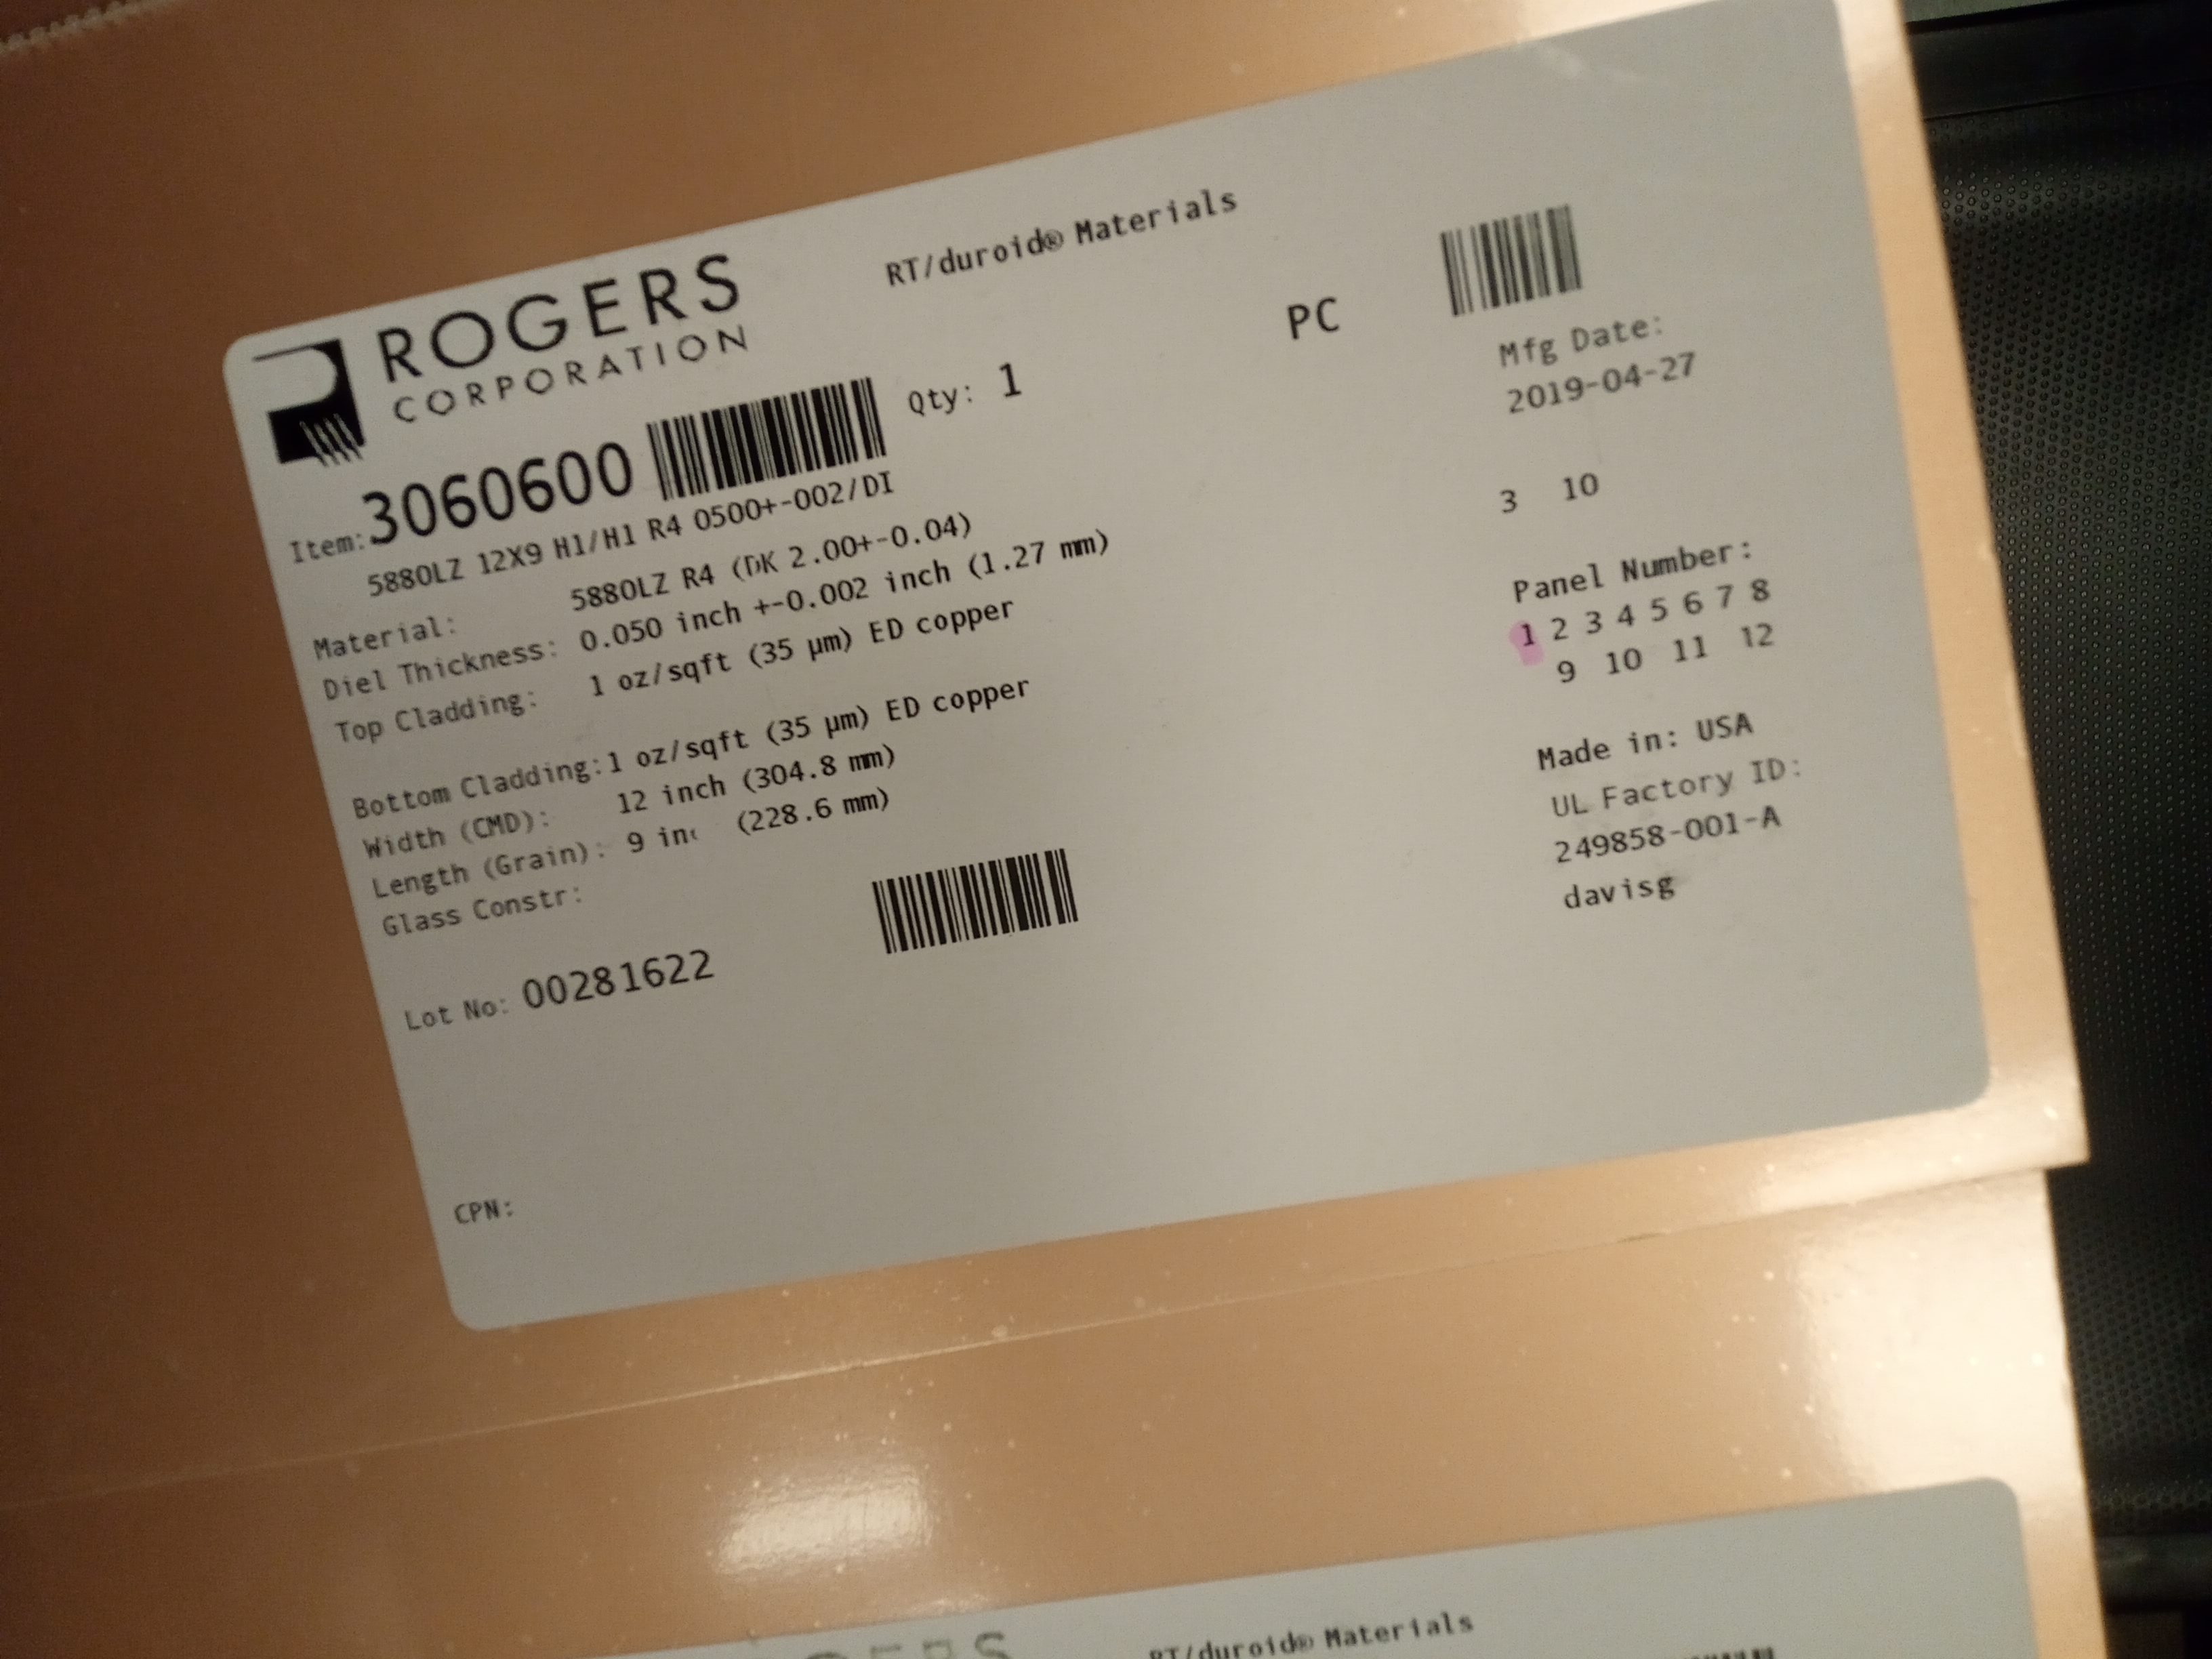
\includegraphics[width=\linewidth]{./img/sustrato.jpg}
\end{minipage}

\begin{minipage}{0.32\linewidth}
    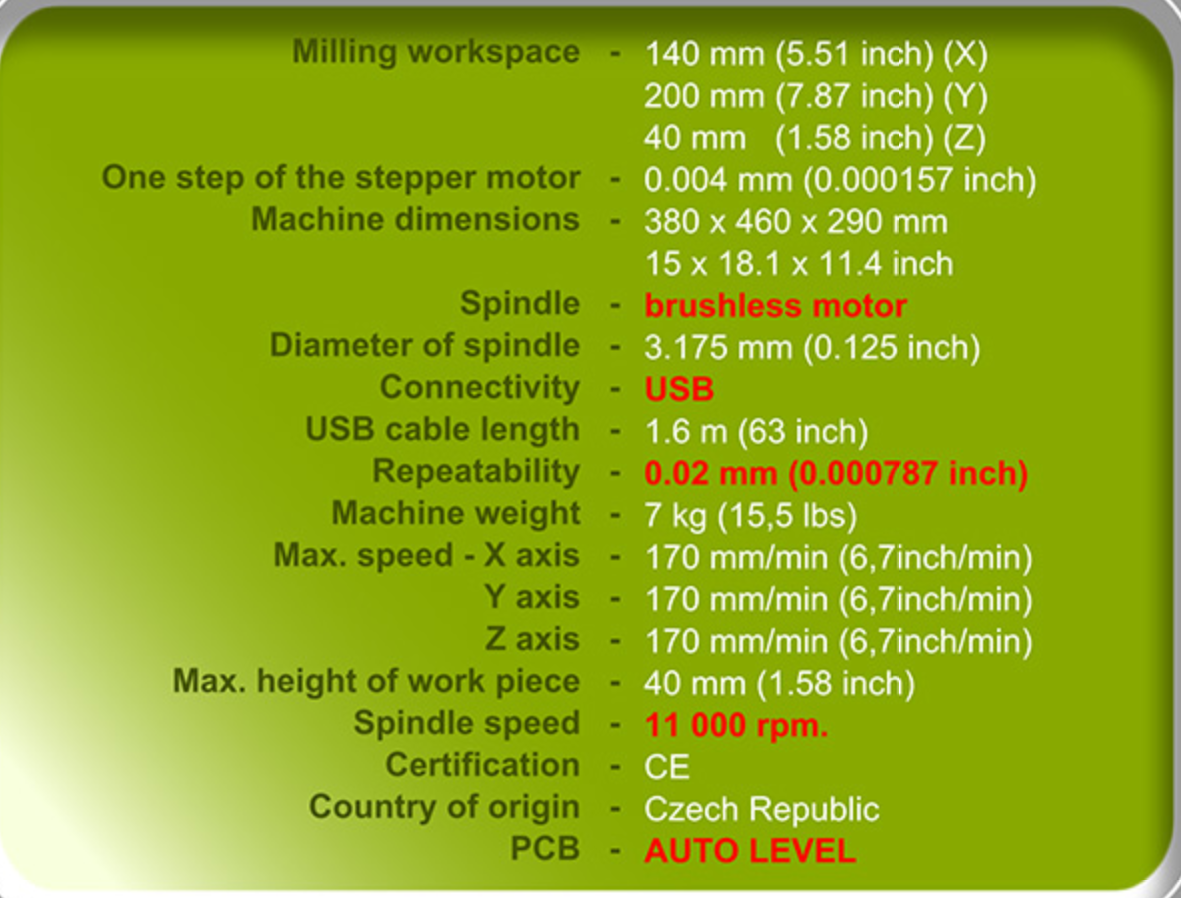
\includegraphics[width=0.8\linewidth]{./img/datasheet_wegstr.png}
\end{minipage}
\begin{minipage}[t]{0.66\linewidth}
La impresión sobre el PCB se hace con un router CNC marca Wegstr con una precisión de $4\mu m$ por paso.
\end{minipage}
\begin{minipage}{0.4\linewidth}
  Las mediciones sobre el proyecto final con un Analizador de redes de dos puertos marca Rohde & Schwarz modelo ZNC3-2Port
\end{minipage}
\begin{minipage}{0.59\linewidth}
  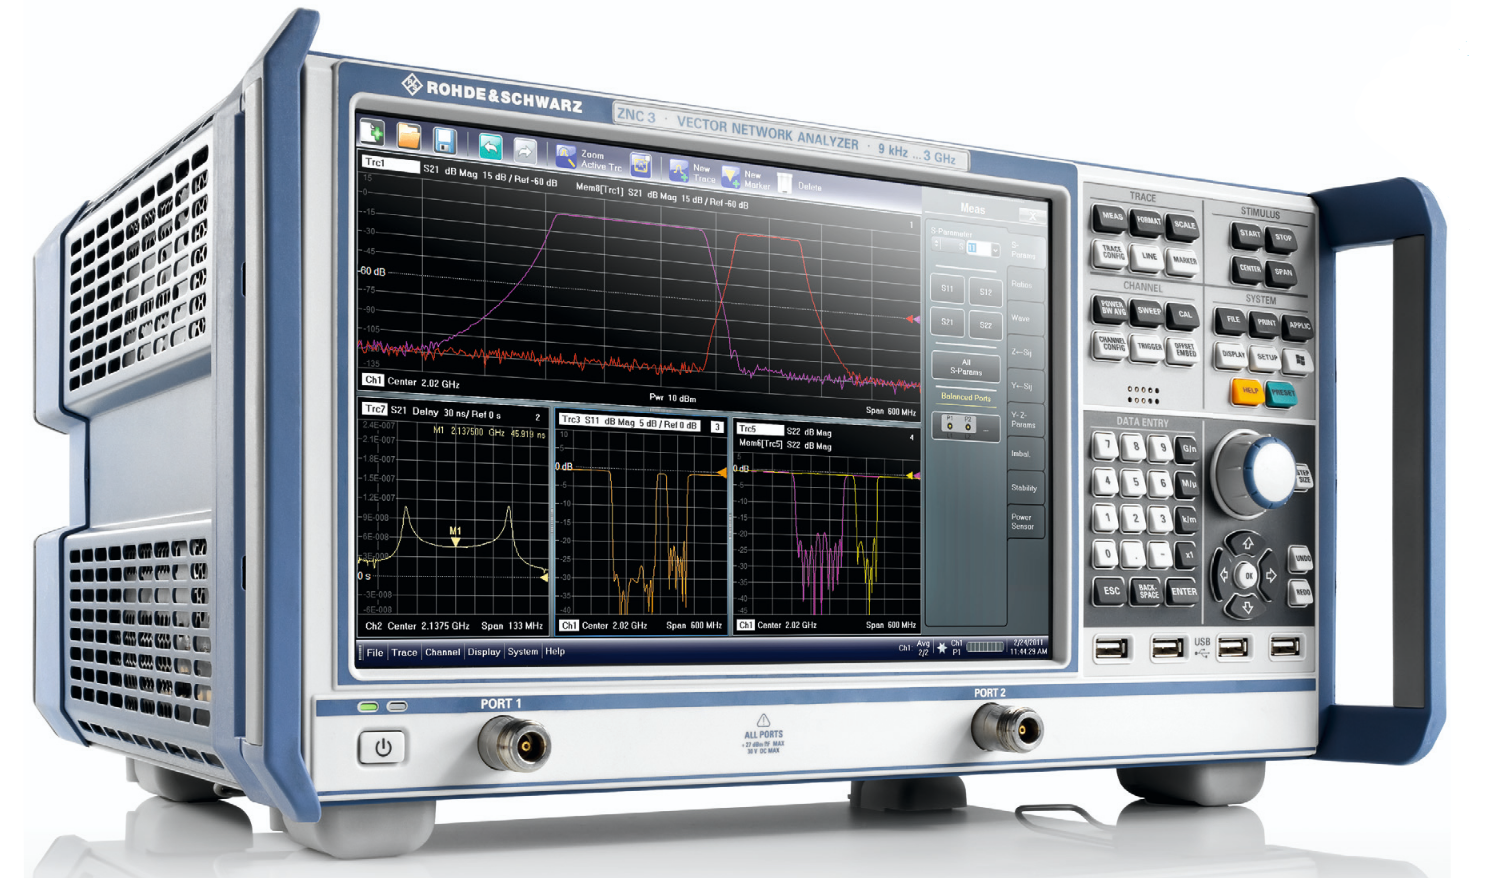
\includegraphics[width=\linewidth]{./img/vna.png}
\end{minipage}

\subsection{Diseño ideal}
Primero hicimos un diagrama funcional y simulamos las relaciones entre entrada y salida.
El esquemático se diseña en ADS y se pone a continuación
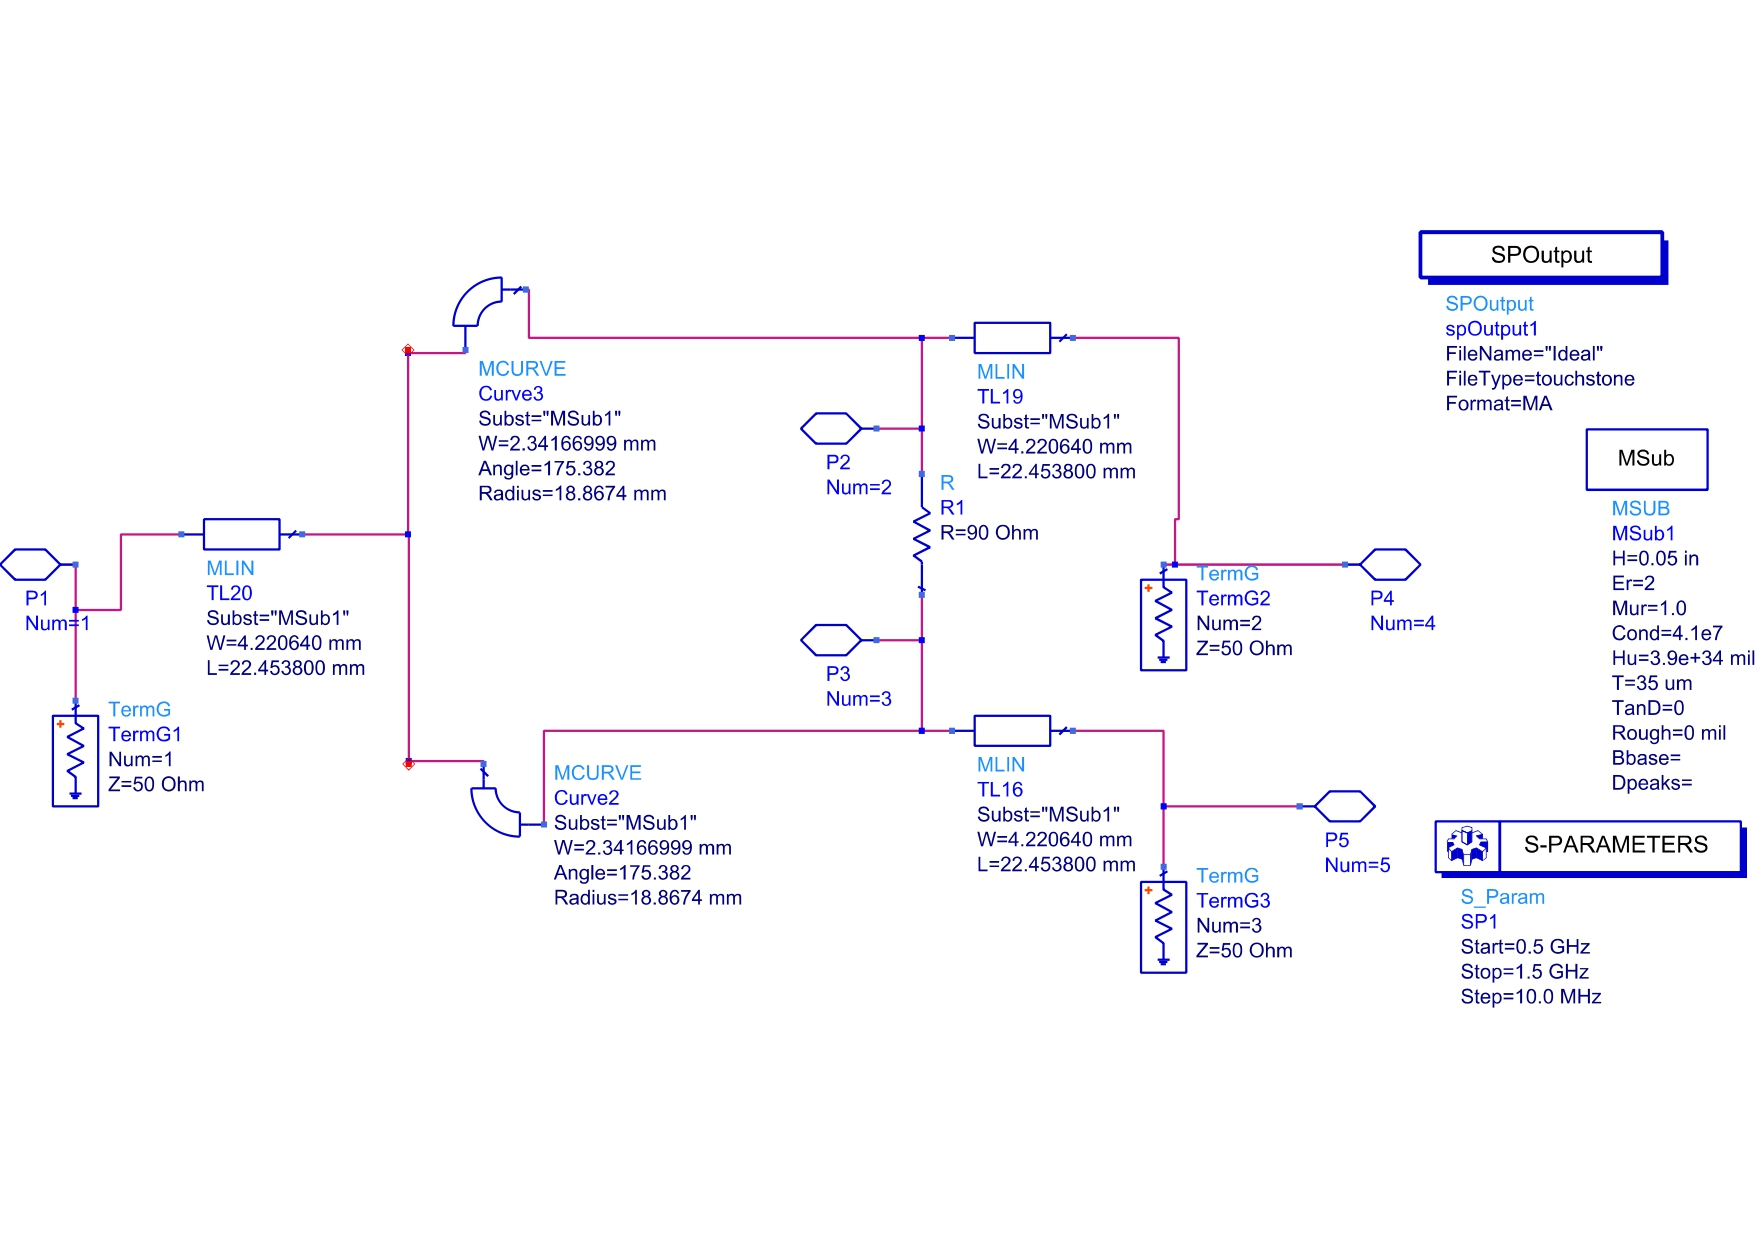
\includegraphics[width = 0.9\linewidth]{./img/ideal.jpg}
Iniciando desde el puerto uno (desde la izquierda) se tienen:

\begin{itemize}
    \item Un tramo calculado para que a $1\text{GHz}$ tenga $1\lambda$ de forma tal de ganar distancia entre el conector y la entrada a los dos transformadores de $\frac{1}{4}\lambda$ sin que haya desfasaje
    \item Dos arcos con un radio calculado de manera tal que su longitud sea $\frac{1}{4}\lambda$. Su ancho de pista se calcula con linecalc para que su impedancia sea $Z = \sqrt{2}Z_0 \approx 70.7\Omega$
    \item Dos puertos con una resistencia en el medio de $90\Omega$. Se elige este valor por limitaciones de stock en laboratorio (ideal sería $100\Omega = 2Z_0$)
    \item Luego el resto hacia la derecha son parámetros necesarios únicamente para ejecutar la simulación
\end{itemize}
Como se ve en la sección de parámetros $S$ del esquemático, la simulación se hace con un barrido de frecuencias entre $0.5$ y $1.5 \text{ GHz}$. Se simula y los resultados se exportan al formato s3p para ser procesados luego con scikit rf en Python (análisis completo en los anexos).
Las líneas verticales gruesas en cada ploteo indican la frecuencia objetivo $1\text{GHz}$ y las líneas punteadas indican el máximo o mínimo encontrado programáticamente a partir de los datos

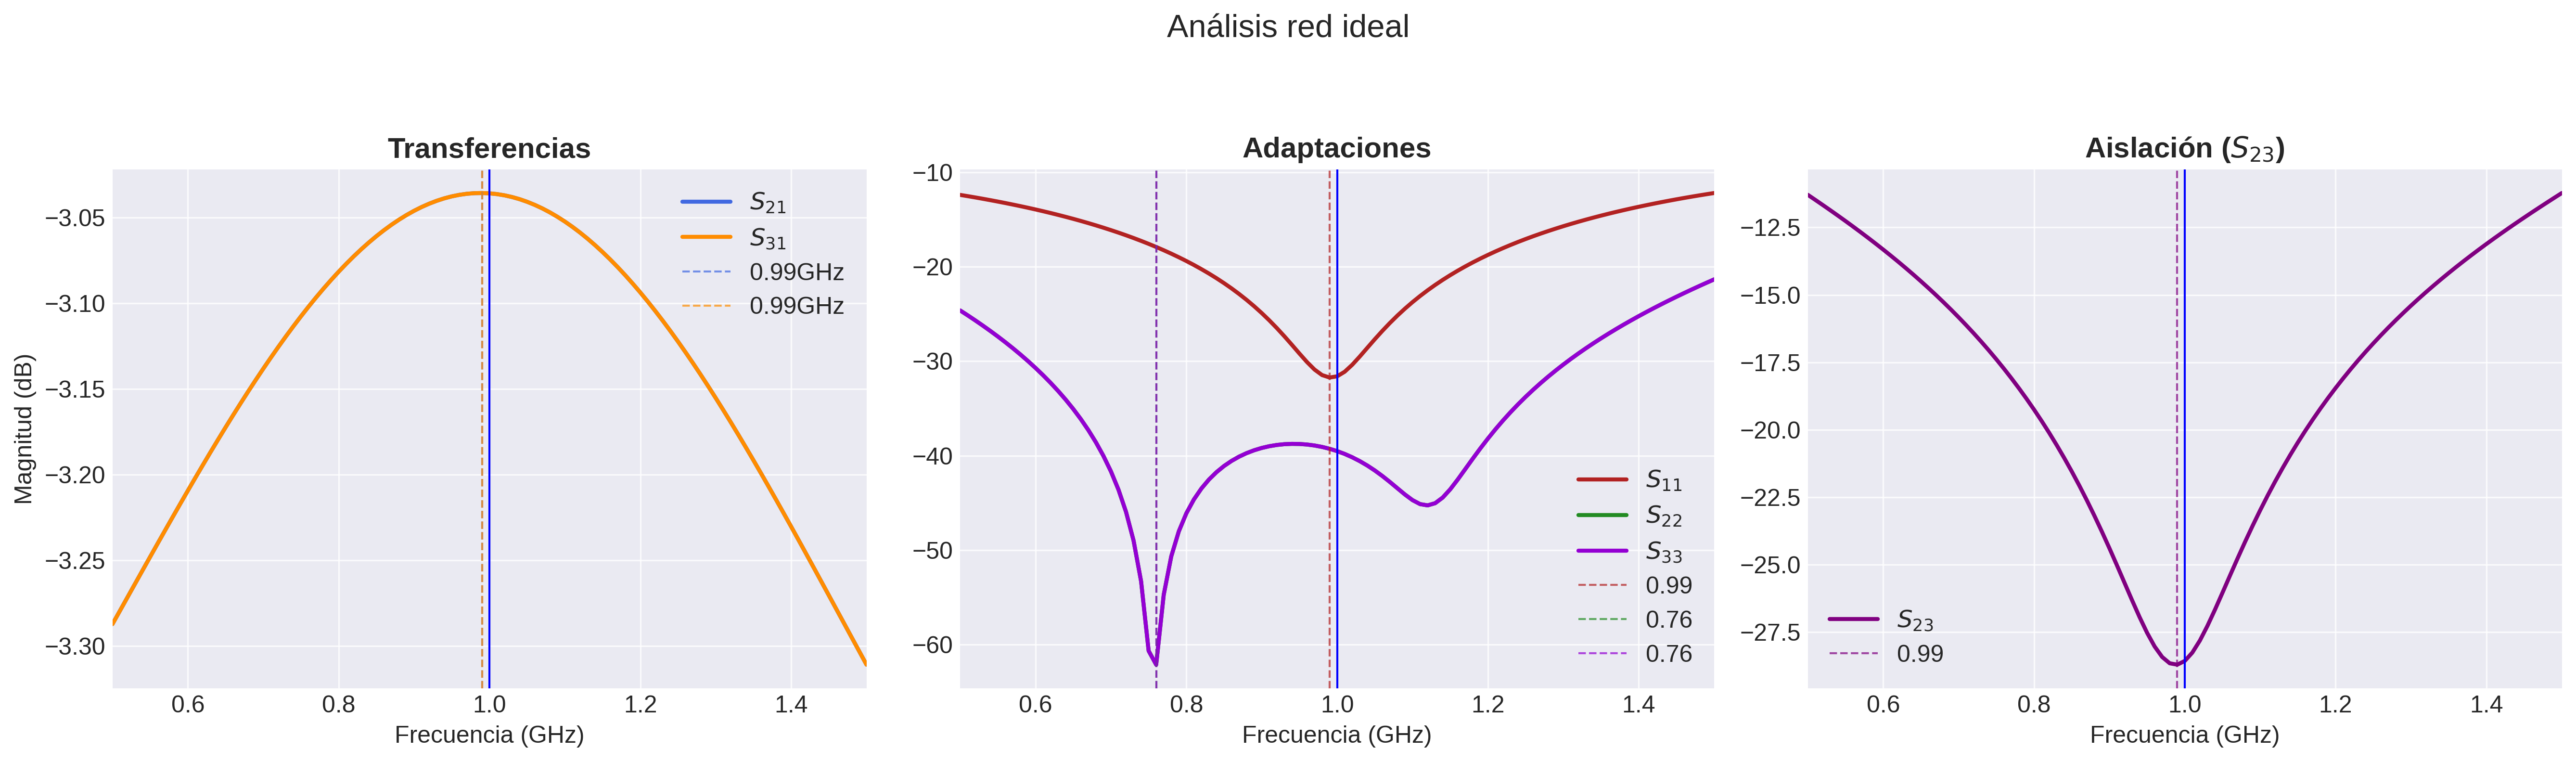
\includegraphics[width=0.9\linewidth]{./img/plot-ideal.png}

\subsection{Diseño físico}
Luego se diseña el bloque físico en ADS a partir del esquemático

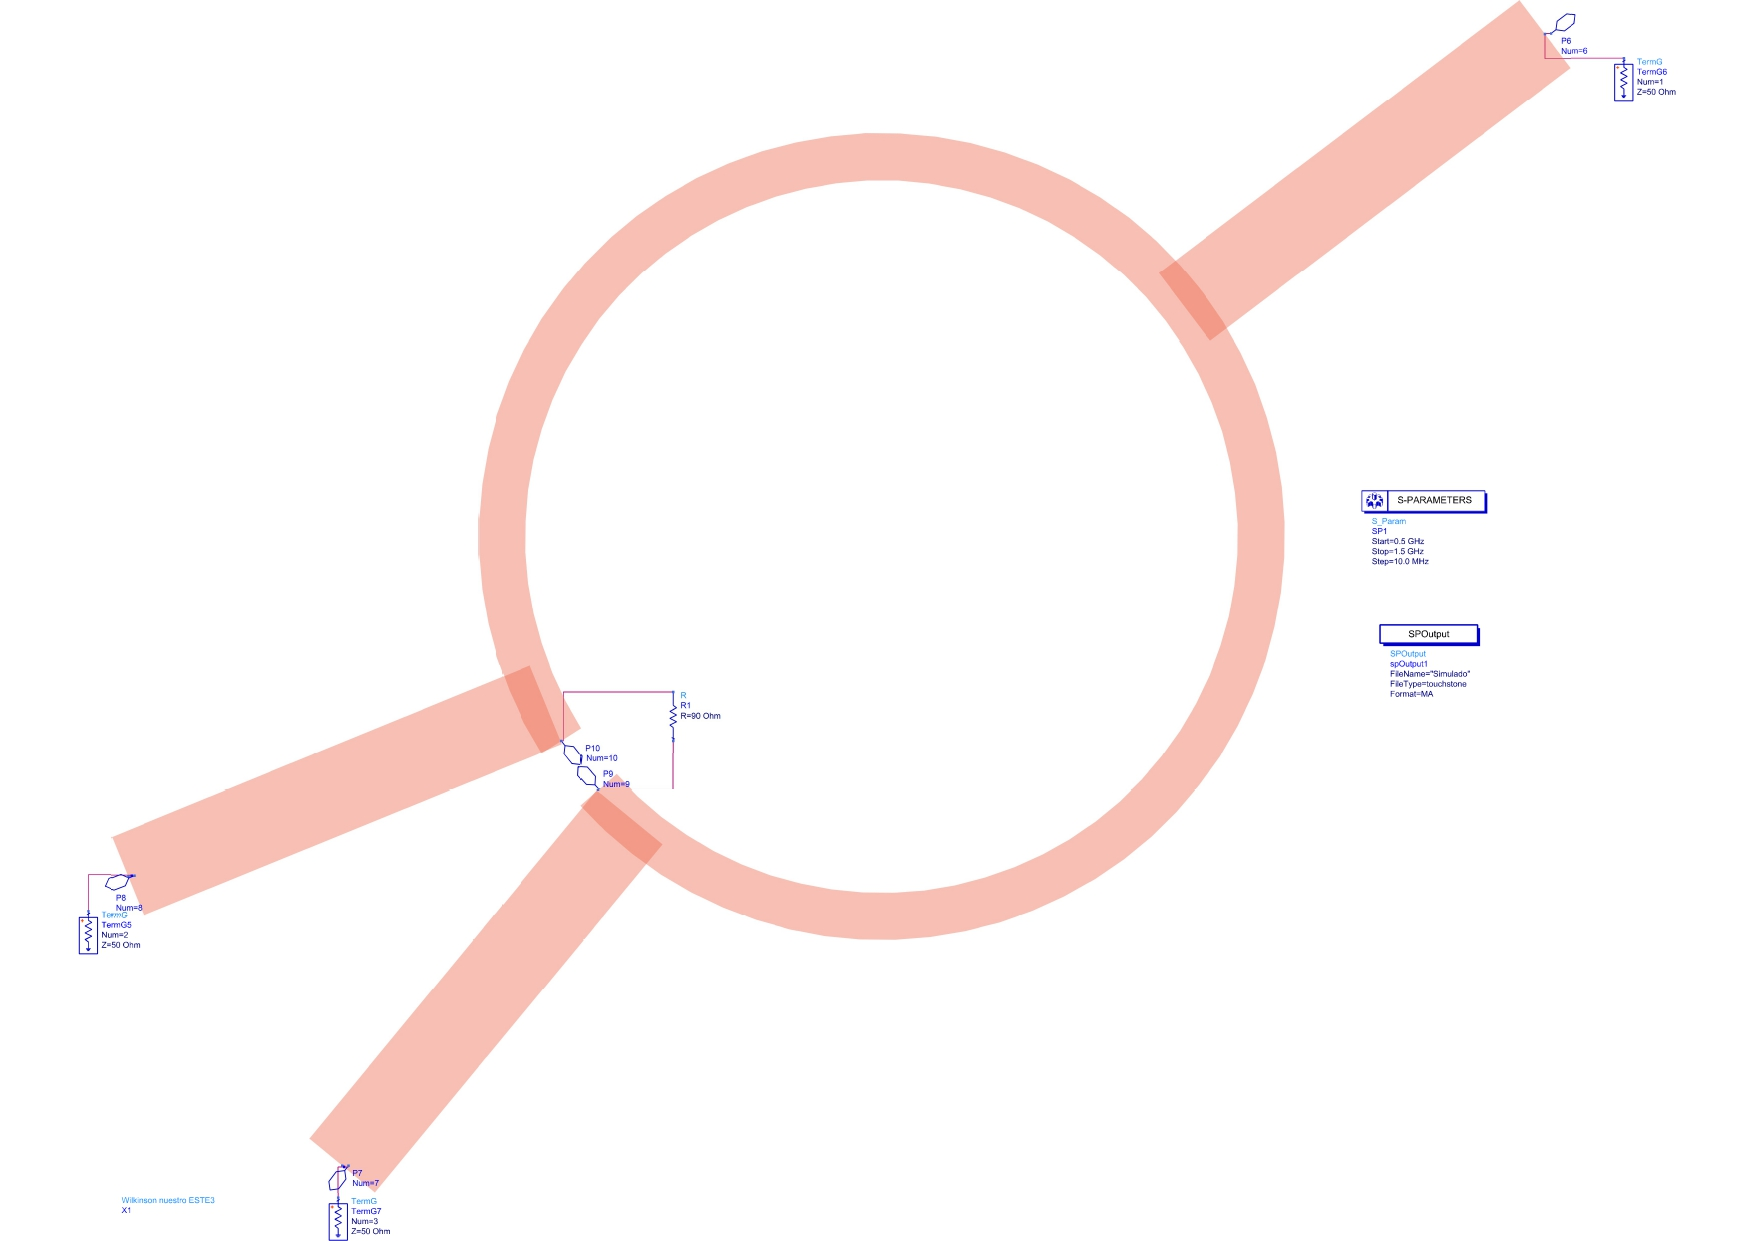
\includegraphics[width=0.6\linewidth]{./img/simulado.jpg}

La optimización de los objetivos de aislación y transferencia se logra mediante una disposición estratégica de las piezas. La selección de dos semi-círculos en lugar de tramos rectos se justifica por dos ventajas técnicas fundamentales:
\begin{itemize}
    \item Maximización de la aislación entre los tramos, reduciendo interferencias.
    \item Eliminación de ángulos agudos en el recorrido de las pistas, lo que mejora el rendimiento electromagnético del diseño.
\end{itemize}
La separación en la salida del transformador hacia los puertos viene dada por el tamaño máximo de una resistencia de radiofrecuencia que conseguimos.

Una vez definido el bloque físico, se realizan simulaciones en ADS para evaluar las transferencias. Los resultados se exportan en formato de parámetros \texttt{s3p} y se analizan mediante la metodología previamente establecida. Los datos obtenidos se presentan a continuación

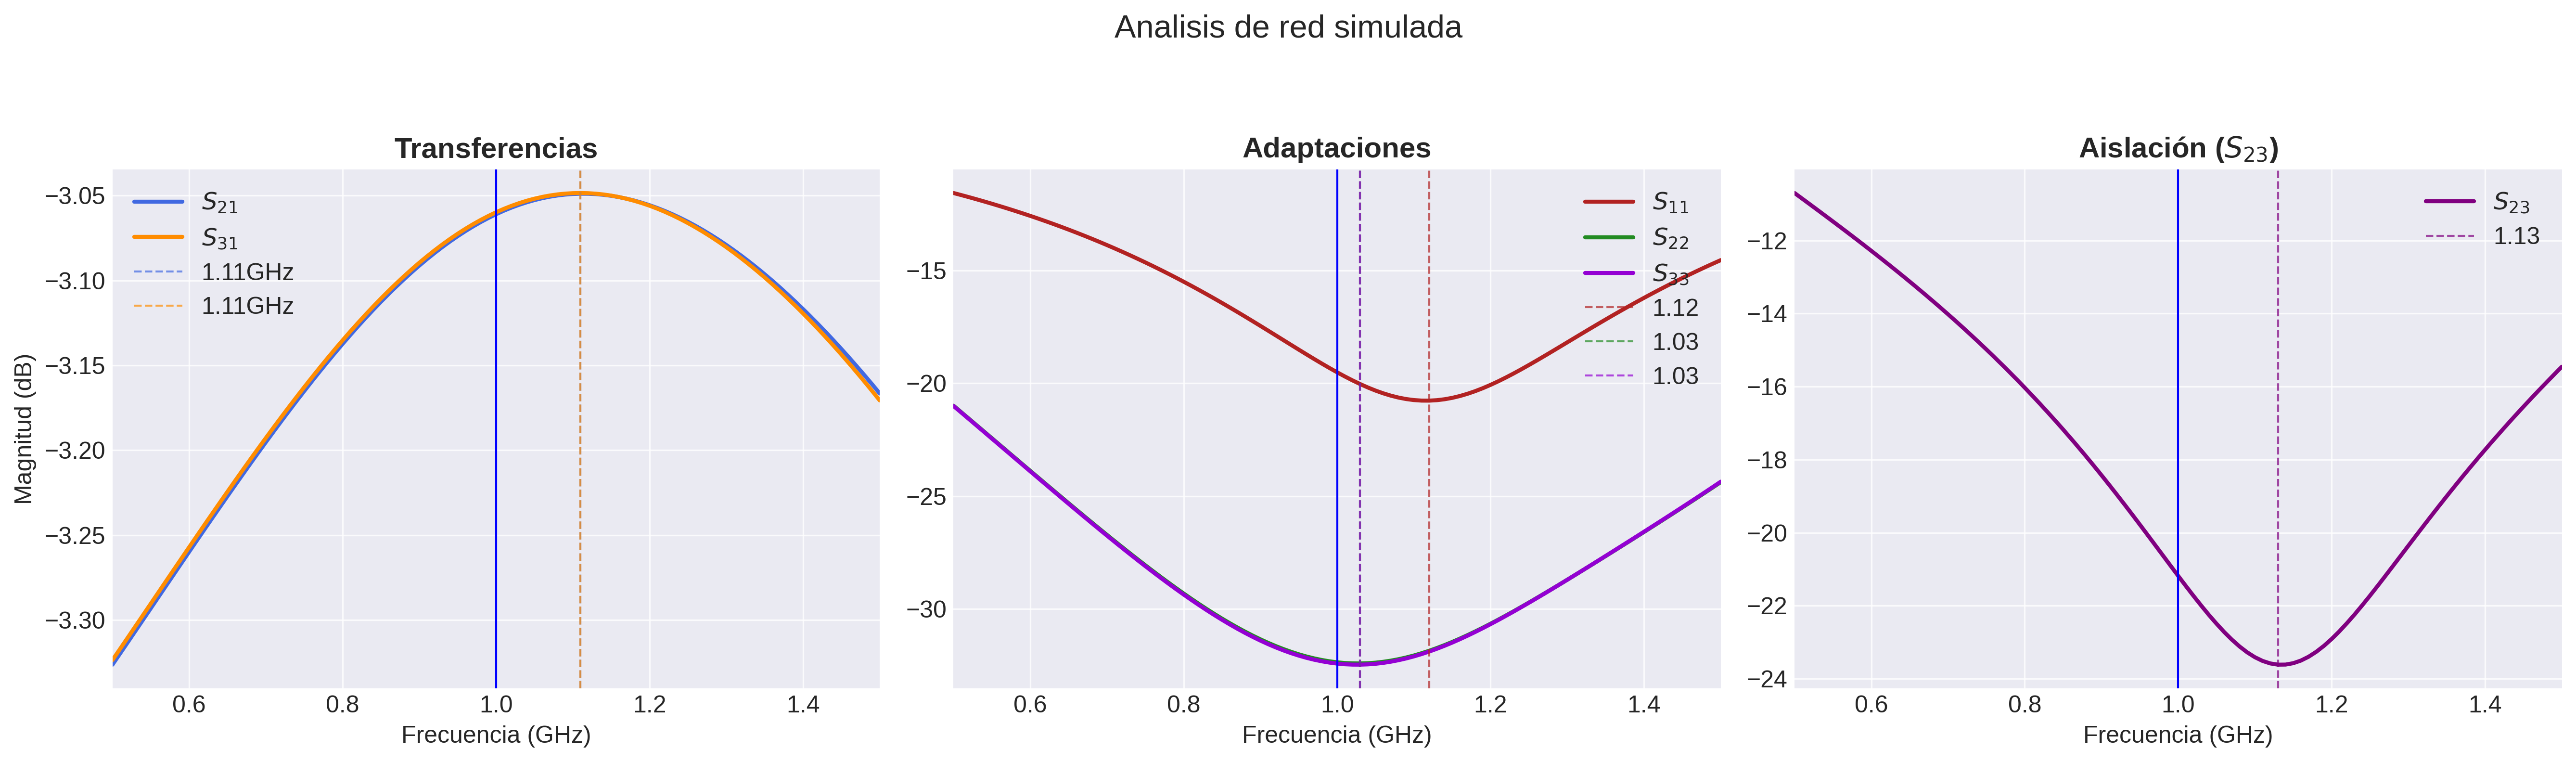
\includegraphics[width=0.9\linewidth]{./img/plot-simulado.png}

Si bien hay un claro desfasaje hacia frecuencias más altas por limitaciónes de tiempo se determina que se mantiene el diseño

\subsection{Construcción física}

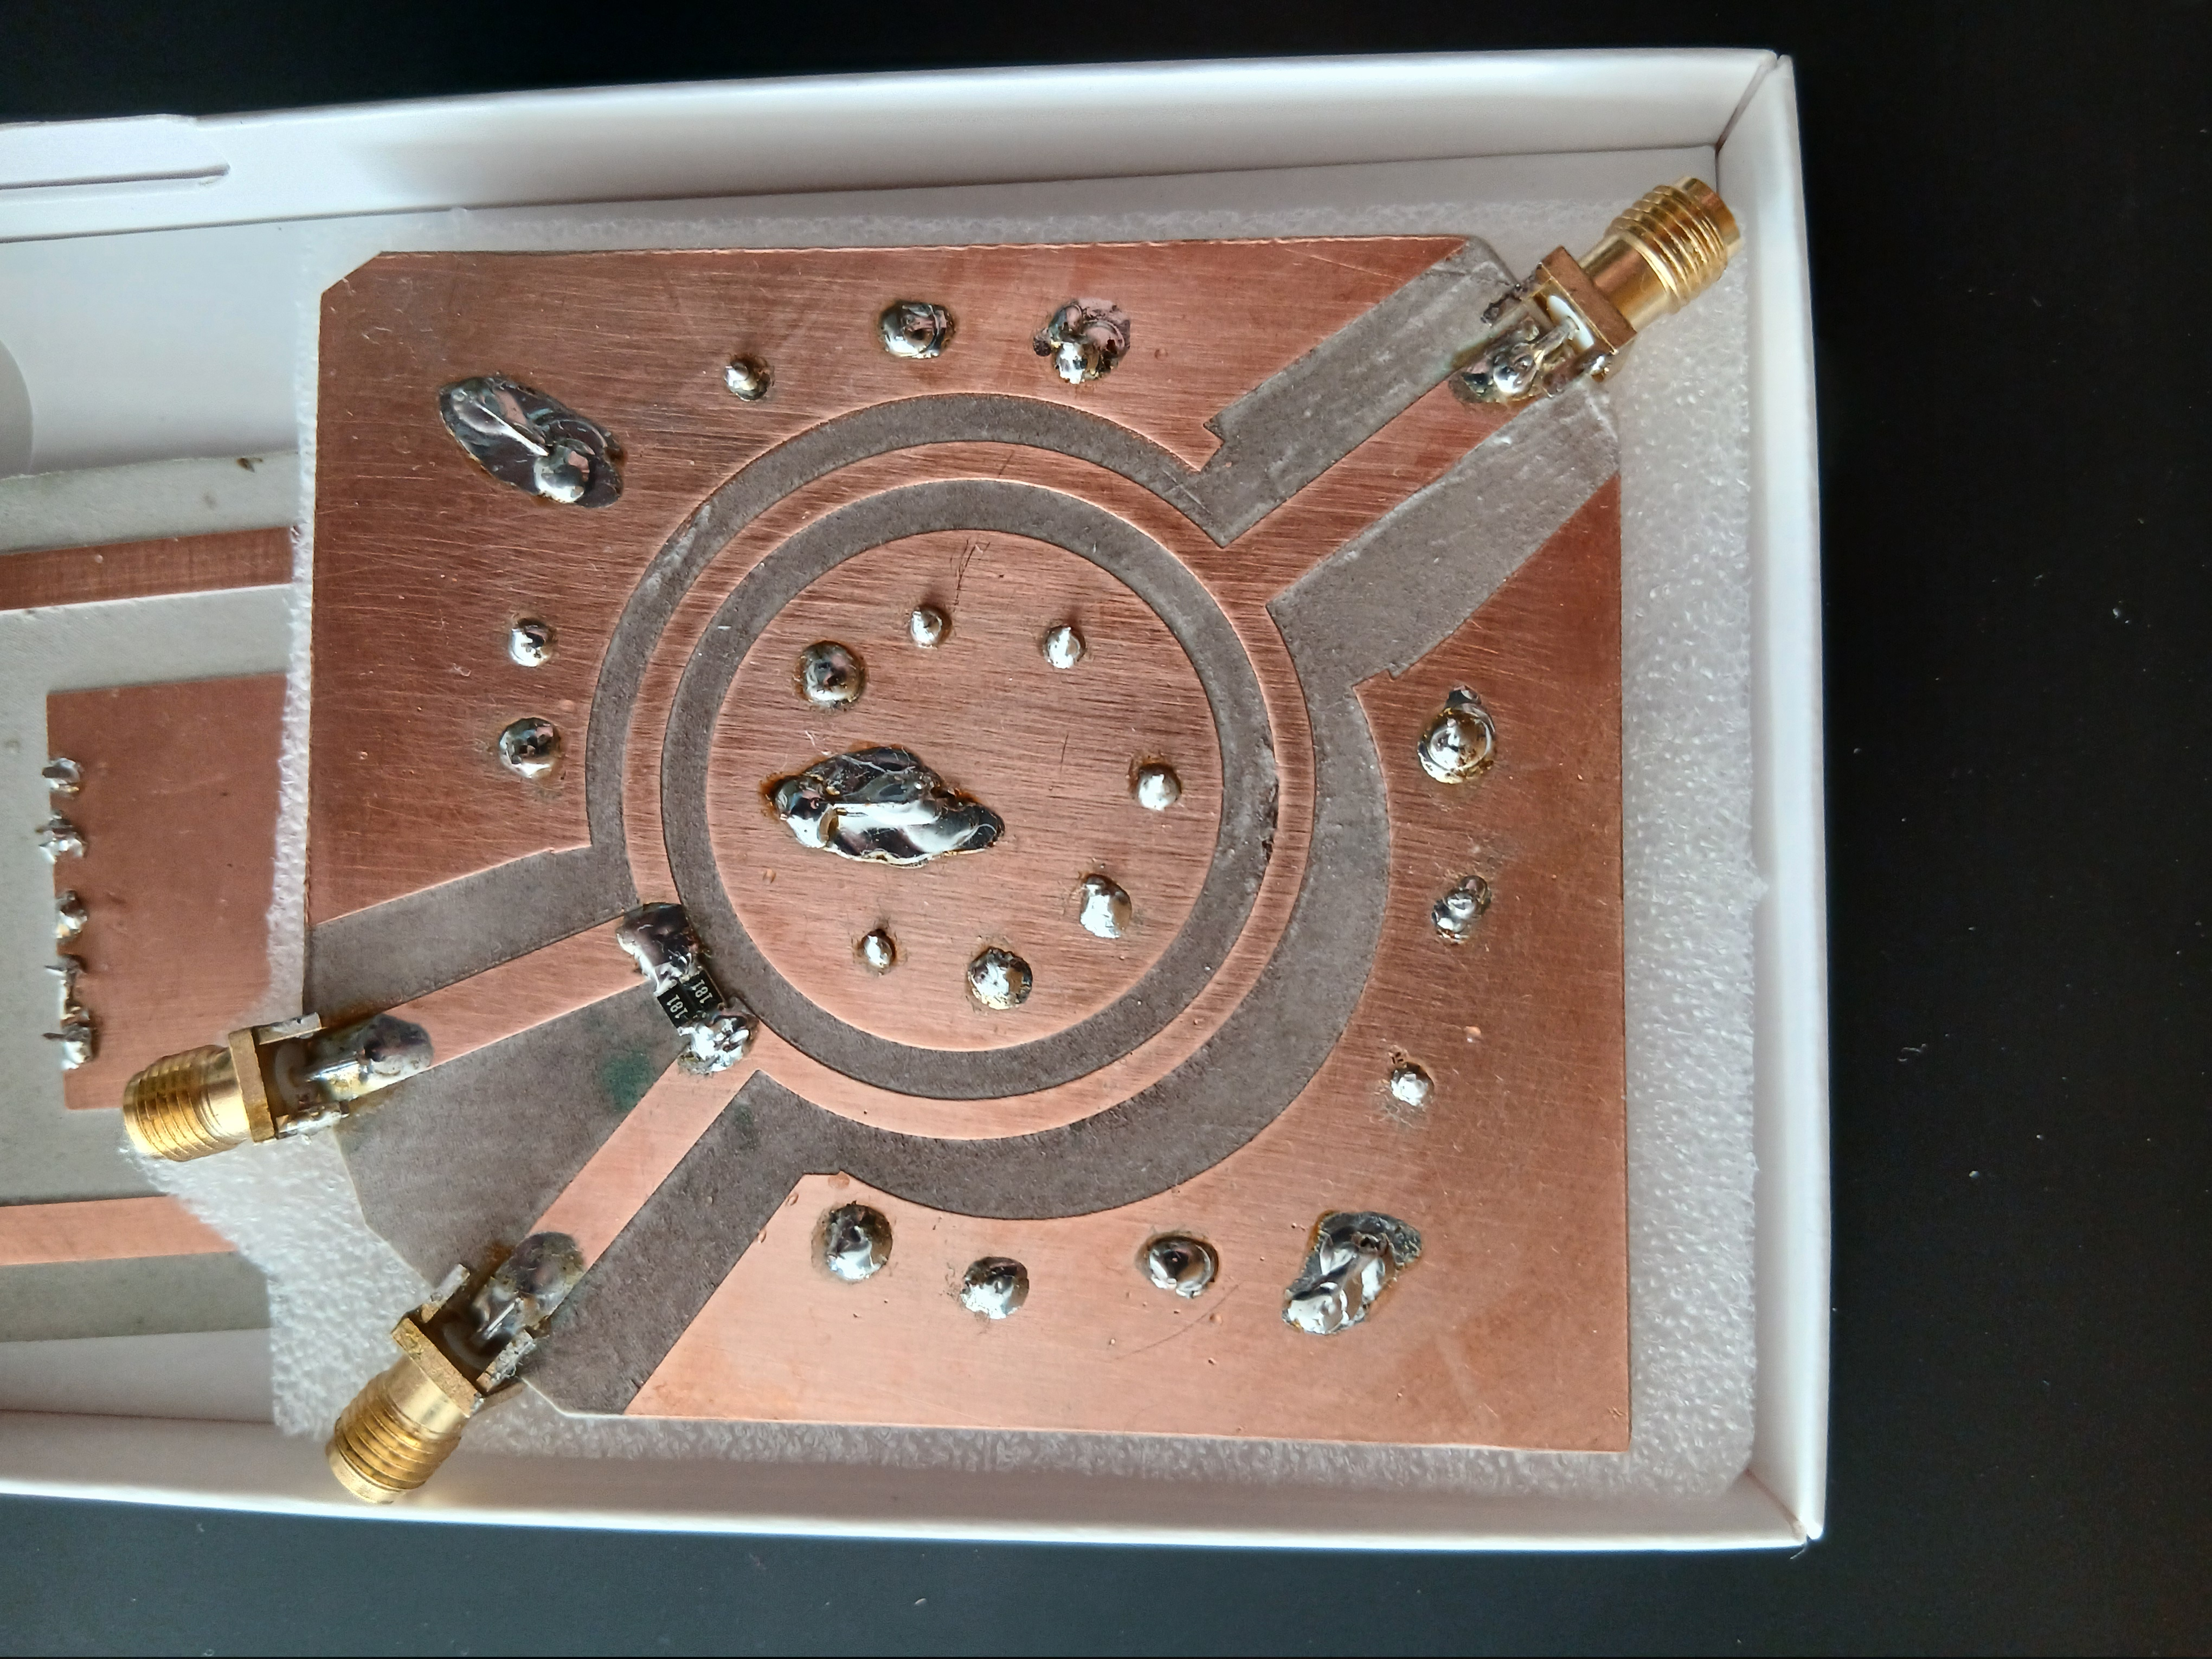
\includegraphics[width=0.7\linewidth]{./img/real.jpg}

\begin{minipage}{0.4\linewidth}
Los datos del diseño se exportan en formato Gerber para su fabricación mediante el router especificado previamente. Durante el ensamblado, los puertos SMA se sueldan manualmente para permitir la conexión con el analizador de redes.
Se añaden conexiónes entre el cobre que rodea a las pistas (por dentro y por fuera) y la tierra (placa de cobre inferior) evitando acoplamientos parásitos
\end{minipage}
\begin{minipage}{0.59\linewidth}
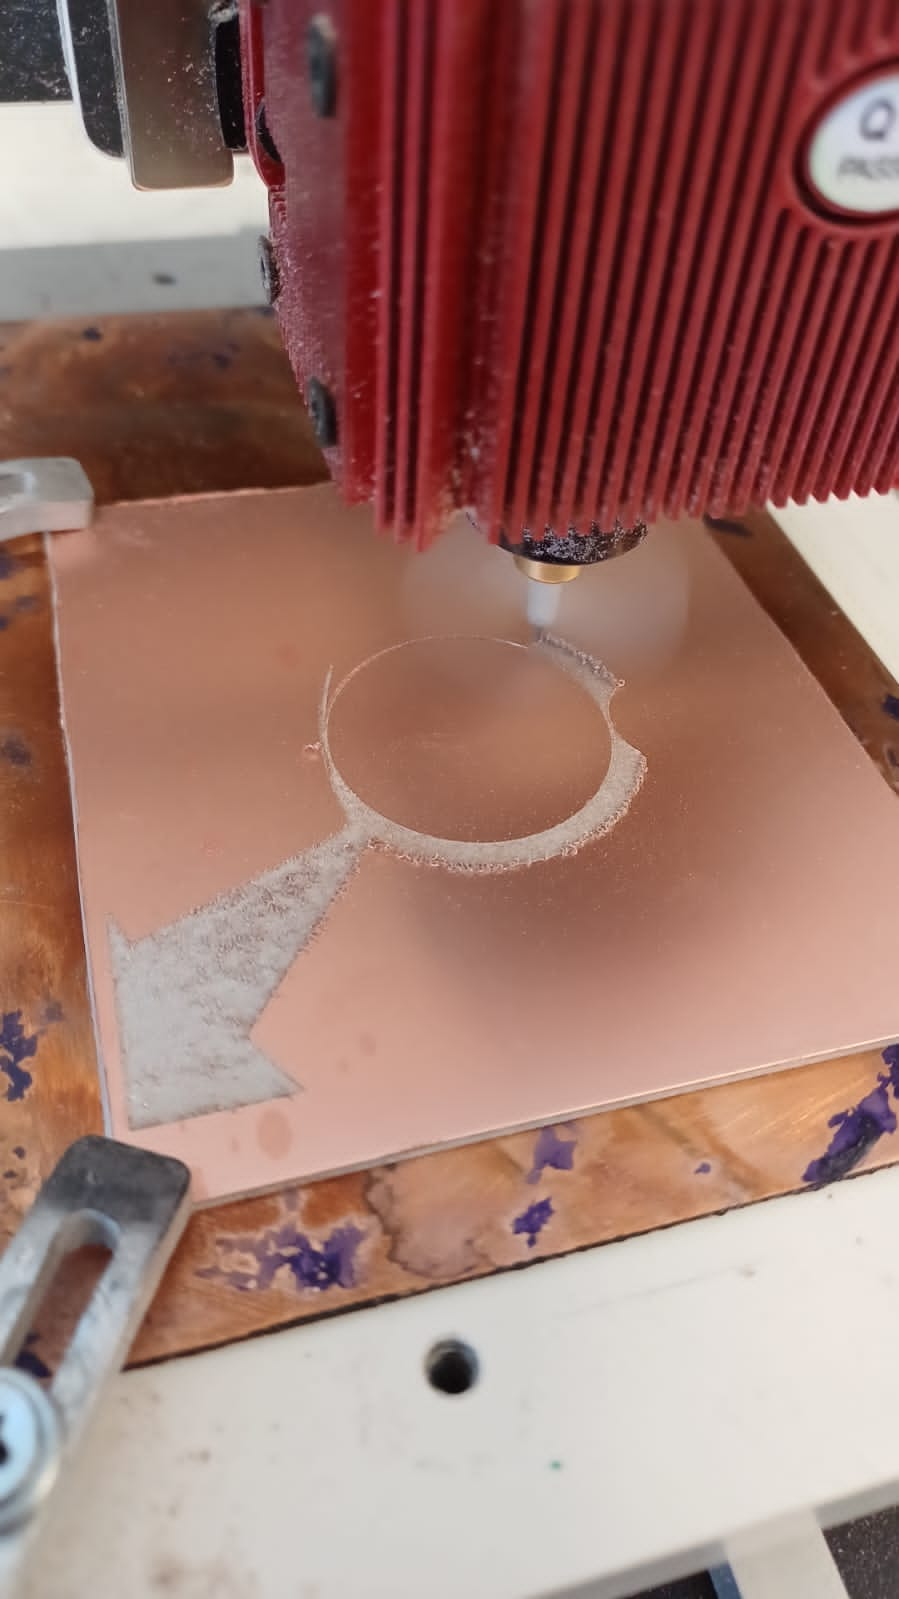
\includegraphics[width=0.49\linewidth]{./img/construccion1.jpg}
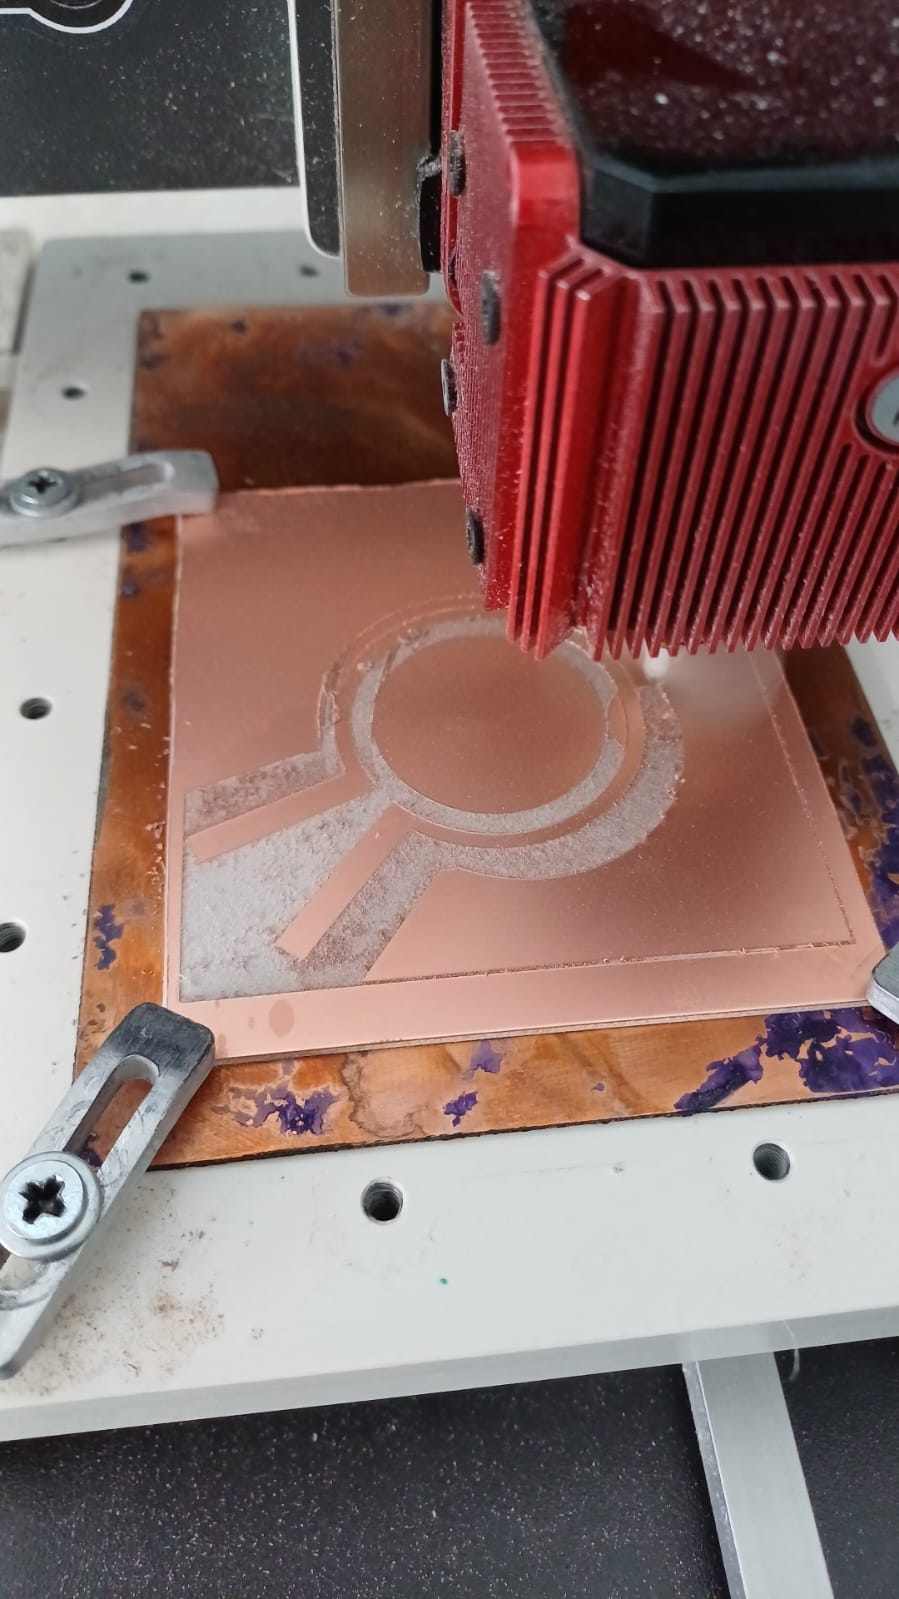
\includegraphics[width=0.49\linewidth]{./img/construccion2.jpg}
\end{minipage}
\subsection{Anexos}
Para más información y documentación técnica, se pueden consultar los siguientes recursos:

\begin{itemize}
    \item Especificaciones del Analizador de Redes Rohde \& Schwarz ZNC 3 - 2 Port: \url{https://scdn.rohde-schwarz.com/ur/pws/dl_downloads/dl_common_library/dl_brochures_and_datasheets/pdf_1/ZNC_dat-sw_en_5214-5610-22_v0302.pdf}
    \item Especificaciones técnicas del router CNC Wegstr: \url{https://www.wegstr.com/specs}
    \item Datasheet del material dieléctrico: \url{https://www.pcb-material.com/datasheet}
\end{itemize}
\end{document}
